\section{Calculus I}

Before we begin introducing mathematical formula, what is a derivative? A derivative calculates the rate of change of a function at any given point. In high school when we learned about the slope of a line -- $y = mx + b$, where $m$ is the slope -- that slope is a derivative. In that context, the derivative is the same at all points because the line is straight. But we often encounter functions that are not a straight line and we care about calculating the slope across values of that function. We can use calculus for this.


\subsection{Sequences and Limits}

A sequence is an ordered list of numbers, e.g.
\begin{equation*}
    \{x_n\} = \{x_1, x_2, ..., x_n\}
\end{equation*}

\noindent Where $x_n$ is a real number that extends from $x_1$ to $x_n$. We usually encounter $n$ extending to $\infty$. Another way to write the series is:
\begin{equation*}
    \{x_n\}_{n=1}^\infty
\end{equation*}

\noindent Central to calculus is the notion of a sequence ``converging to a limit'', generally where $n \rightarrow \infty$ or $n \rightarrow 0$. This is written as:
\begin{equation*}
    \lim_{n \rightarrow \infty} y_n = L
\end{equation*}

\noindent where L is the limit. Let's visualize for an arbitrary function, $f(x) = \frac{x + 10}{x}$:

\begin{center}
    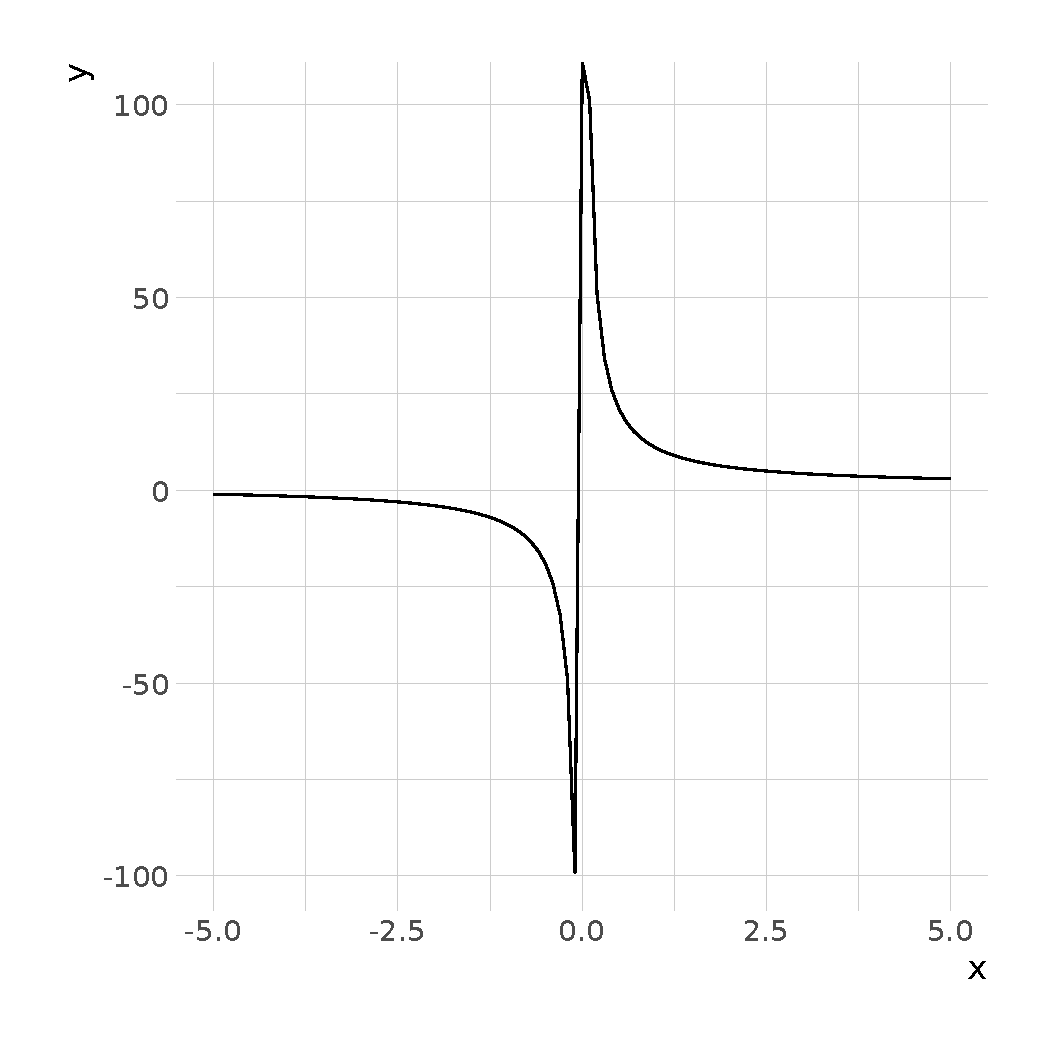
\includegraphics[scale = 0.55]{figures/limit.pdf}    
\end{center}

\noindent We can see that as $x \rightarrow \infty$ the value of $f(x)$ stabilizes. Indeed:

\begin{equation*}
    \lim_{x \rightarrow \infty} \frac{x + 10}{x} = 
    \lim_{x \rightarrow \infty} \left(1 + \frac{10}{x}\right) = 
    \underbrace{\lim_{x \rightarrow \infty} 1}_1 + \underbrace{\lim_{x \rightarrow \infty} \frac{10}{x}}_0 = 1
\end{equation*}

\noindent This gives us a limit of 1.

\subsection{Derivatives and the Difference Quotient}

The derivative is the rate of change of $f(x)$ at any $x$. For a straight line, i.e $y = mx + b$, the derivative is constant at all points. But for a nonlinear function, i.e. $y = 2x^4$, the rate of change varies across x.

\begin{figure}[ht]
    \centering
        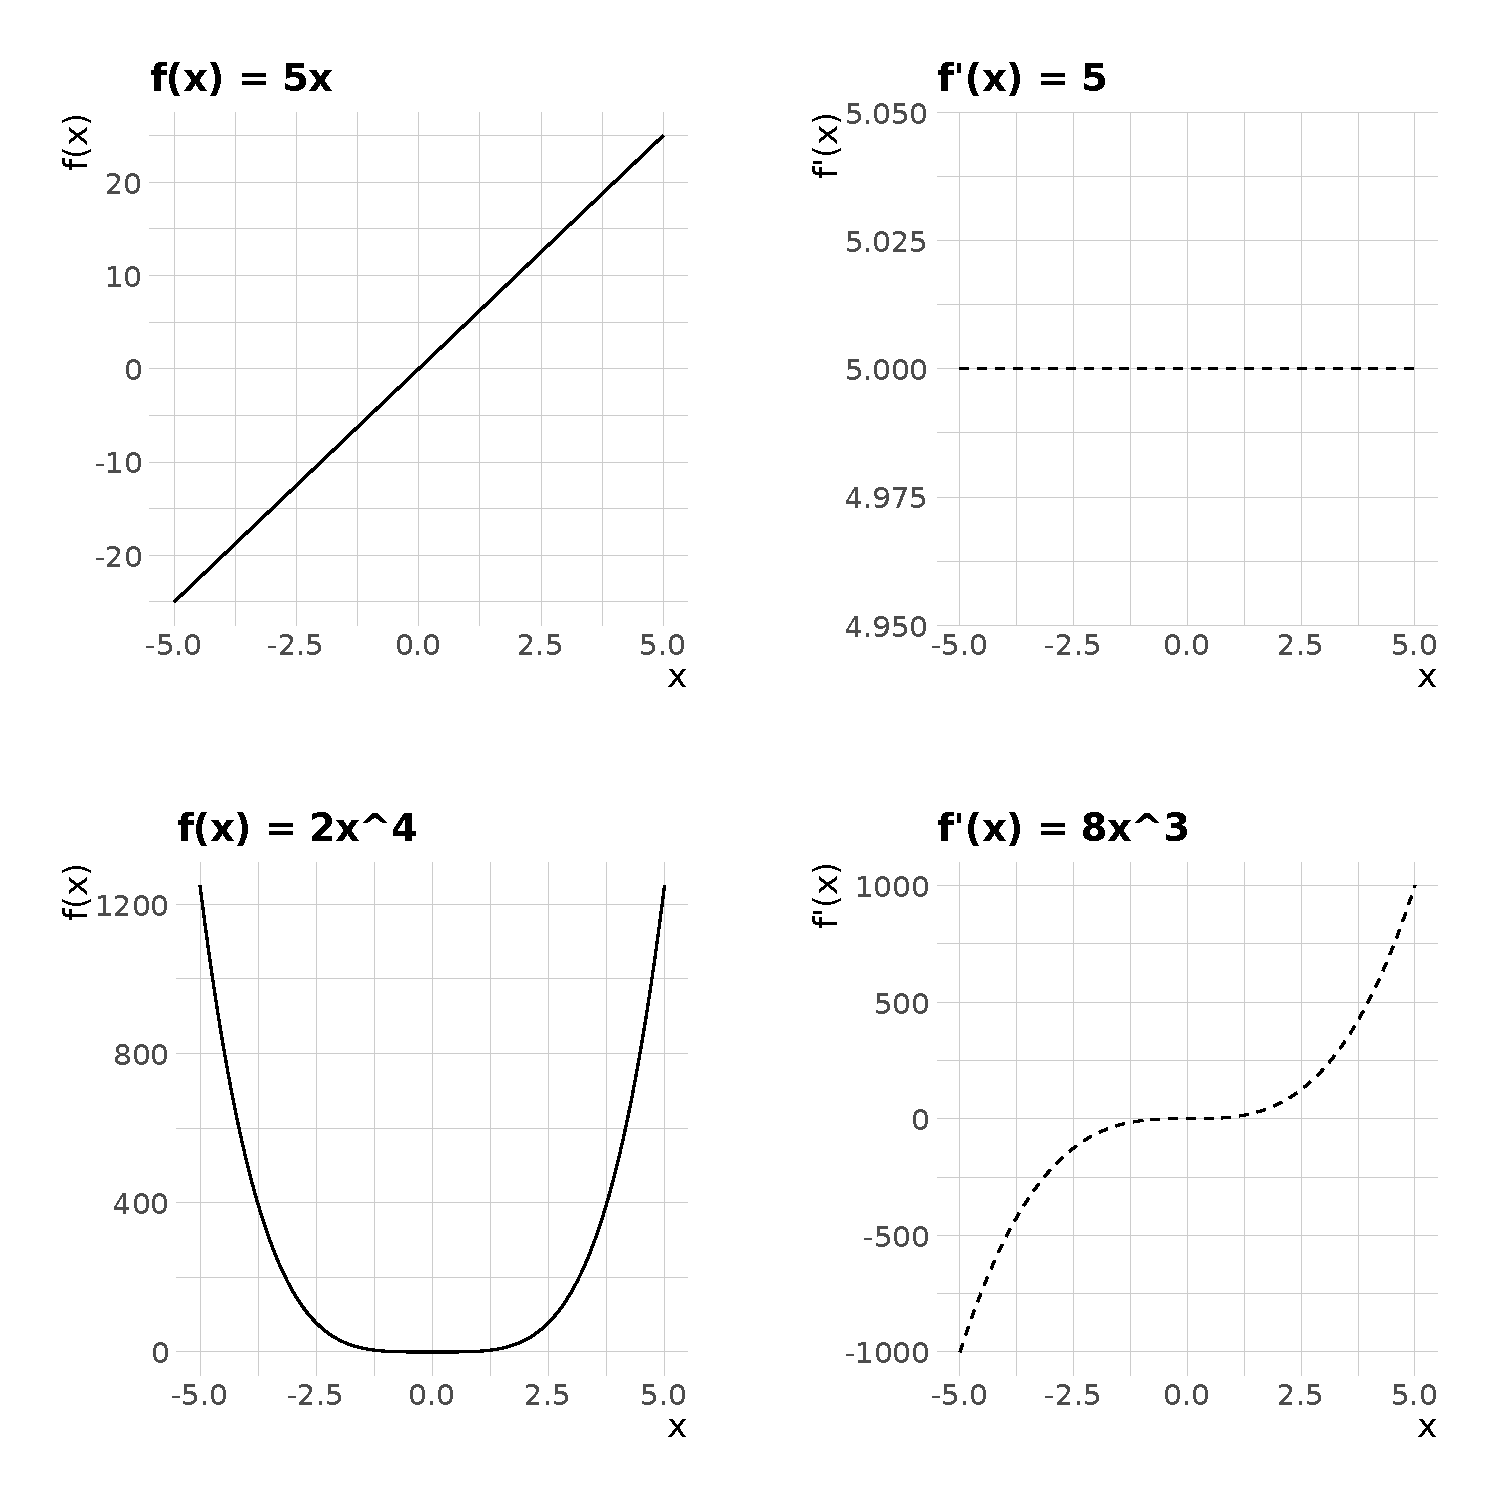
\includegraphics[scale = 0.55]{figures/derivs.pdf}    
    \caption{Functions and their derivatives}
    \label{fig:deriv}
\end{figure}

\noindent Now, let's introduce how we produce a derivative. Let $f$ be a function with an open interval that contains $x$. Let $h$ be the interval where $f(x)$ changes. Below we are simply calculating rise over run at each specified interval.

\begin{equation*}
    \frac{d}{dx}f(x) = 
    \lim_{\Delta x \rightarrow 0} \frac{f(x + \Delta x) - f(x)}{\Delta x} 
\end{equation*}

\noindent The numerator represents the change in $f(x)$ as $\Delta x$ approaches 0 and the denominator is the change in $\Delta x$ -- or the change in $x$. We generally see two notations for derivatives:
\begin{itemize}
    \item Lagrange: $f'(x)$
    \item Leibniz: $\frac{d}{dx}y = \frac{dy}{dx}$
    \begin{itemize}
        \item The change in $y$, given change in $x$.
    \end{itemize}
\end{itemize}

\noindent Side-note, on the problem set, when we are asked about the difference quotient as a function of $x + \Delta x$, think about how a specified function would look if it were plugged in for $f(x)$ and $f(x + \Delta x)$.

\subsection{Rules for Derivatives}

\begin{itemize}
    \itemsep-0.5em 
    \item Power rule:
    \begin{itemize}
        \item $y = f(x) = ax^n$, $f'(x) = nax^{n-1}$
    \end{itemize}
    \item Constant multiplier rule:
    \begin{itemize}
        \item $f(x) = ax$, $f'(x) = a$
    \end{itemize}
    \item Constant rule:
    \begin{itemize}
        \item $f(x) = a$, $f'(x) = 0$
    \end{itemize}
    \item Summation rule:
    \begin{itemize}
        \item $f(x) = g(x) + h(x)$, $f'(x) = g'(x)h'(x)$
    \end{itemize}
    \item Product rule:
    \begin{itemize}
        \item $f(x) = g(x)h(x)$
        \item $f'(x) = g'(x)h(x) + g(x)h'(x)$
    \end{itemize}
    \item Quotient rule:
    \begin{itemize}
        \item $f(x) = g(x)/h(x)$
        \item $f'(x) = \frac{g'(x)h(x) - g(x)h'(x)}{[h(x)]^2}$
    \end{itemize} 
    \item Chain rule:
    \begin{itemize}
        \item $f(x) = h[g(x)]$
        \item $f'(x) = h'[g(x)] \cdot g'(x)$
    \end{itemize}
    \item Exponent rule:
    \begin{itemize}
        \item $f(x) = a^x$
        \item $f'(x) = a^x(ln(a))$
        \item $f(x) = e^x$, $f'(x) = e^x$
    \end{itemize}
    \item Logarithm rule:
    \begin{itemize}
        \item $f(x) = \text{log}_a x$
        \item $f'(x) = \frac{1}{x\text{ln}a}$
        \item Natural log: $f(x) = ln(x)$, $f'(x) = \frac{1}{x}$
    \end{itemize}
\end{itemize}

\subsection{Derivative Examples}

\begin{enumerate}
    \item $f(x) = 40x^{400}$
    \begin{itemize}
        \item $f'(x) = 400\cdot40x^{399} = 16000x^{399}$
    \end{itemize}
    \item $f(x) = 16x$
    \begin{itemize}
        \item $f'(x) = 16$
    \end{itemize}
    \item $f(x) = 1000$ 
    \begin{itemize}
        \item $f'(x) = 0$
    \end{itemize}
    \item $f(x) = 3x^{100} + 5x^2$
    \begin{itemize}
        \item $f'(x) = 300x^{99} + 10x$
    \end{itemize}
    \item $f(x) = (3x + 5)(9x + 2)$
    \begin{itemize}
        \item $f'(x) = 3(9x + 2) + 9(3x + 5)$
    \end{itemize}
    \item $f(x) = \frac{3x + 5}{9x + 2}$
    \begin{itemize}
        \item $f'(x) = \frac{3(9x + 2) - 9(3x + 5)}{(9x + 2)^2}$
    \end{itemize}
    \item $f(x) = 20(x + 3)^{10}$
    \begin{itemize}
        \item $f'(x) = 200(x + 3)^9 \cdot 1$
    \end{itemize}
    \item $f(x) = 20(x^3 + 3x)^{10}$
    \begin{itemize}
        \item $f'(x) = 200(x^3 + 3x)^9 \cdot (3x^2 + 3)$
    \end{itemize}
    \item $f(x) = 20[(x + 3)^3 + 4x]^{10}$
    \begin{itemize}
        \item $f'(x) = 200[(x + 3)^3 + 4x]^9 \cdot g'(x)$
        \item $g'(x) = 3(x + 3)^2 \cdot 1 +  4$
        \item $f'(x) = 200[(x + 3)^3 + 4x]^9 \cdot 3(x + 3)^2 + 4$
    \end{itemize}
    \item $f(x) = e^{\sqrt{x}}$, 
    $f'(x) = e^{x^{\frac{1}{2}}} \cdot (\frac{1}{2}x^{-\frac{1}{2}})$
    \item $f(x) = a^{\sqrt{x}}$, 
    $f'(x) = a^{\sqrt{x}}ln(a) \cdot (\frac{1}{2}x^{-\frac{1}{2}})$
    \begin{itemize}
        \item Keep in mind for the problem set.
    \end{itemize}
    \item $f(x) = ln(3x^2 + 3x + 3)$,
    $f'(x) = \frac{1}{3x^2 + 3x + 3} \cdot 6x + 3 = 
    \frac{6x + 3}{3x^2 + 3x + 3}$
\end{enumerate}